\documentclass{article}
%\documentclass[twocolumn]{article}
\usepackage{fullpage}
\usepackage{amsmath}
\usepackage{apacite}
\usepackage{url}
\usepackage{graphicx}
\usepackage{subfigure}
%\usepackage{paralist}
%\usepackage{mdwlist}
\newcommand{\comment}[1]{}
\bibliographystyle{apacite}

\usepackage{float}
\newfloat{Algorithm}{h!}{}{}

% program-related commands
\usepackage{program}
\renewcommand{\|}{\origbar} % use this instead of '|' because program package redefines '|'
\renewcommand{\WHILE}{\mbox{{\bf while} }\tab}
\renewcommand{\FOR}{\mbox{{\bf for} }\tab}
\renewcommand{\IF}{\mbox{{\bf if} }\tab}
\newcommand{\IN}{\mbox{ {\bf in} }}

\newcommand{\xyspace}{{\em xy} space}

\begin{document}
\title{Object Detection with AGiNG}
\author{Andrew Stromme \& Ryan Carlson}
\date{May 14, 2010}
\maketitle

\begin{abstract}
\end{abstract}

\section{Introduction}

Talk about using a modified Growing Neural Gas to track objects. Why is this cool? $-->$ Don't need any type of edge detection. Computationally inexpensive (amortized). We see this as a replacement for the 'blobify' filter.

\section{Related Work}

Talk about Growing Neural Gas papers by Fritzke and maybe the CBIM paper by Meeden. Also mention some previous attempts at object tracking -- Canny/Sobel edge detection. AdaBoost?

\section{Goals}

%We want to create a Growing Neural Gas that can identify objects and then have the AIBO track it. Talk about limitations of blobify and how this improves it.
At the broadest level of abstraction, our task is object recognition and tracking using a Growing Neural Gas. We provide an image for the GNG to categorize, and the GNG identifies the objects. In the case of a movie, the GNG must be able to update and adapt to the scene. Objects moving across a canvas need to be identified from one frame to another. To test the algorithm's capacity for tracking, we used sets of simple, computer generated images along with real-world images taken with a camera. Additionally, we created computer generated sequences of images that served as a simple movie. On the other end, we ran the GNG on real-time input coming from a webcam and got encouraging results. We also interfaced with the AIBO and were able to give it appropriate commands given an object to follow moving the scene.

The rest of the paper is organized as follows. Section \ref{sec:GNG} details our implementation of the Growing Neural Gas algorithm in C++. Since our object detection needed to happen in real time, this was an important first task making the GNG very fast. In section \ref{sec:creatingGNG} we discuss the creation and visualization of the GNG. The inputs and the reasoning behind some basic decisions is described. We write about a number of modifications to the GNG algorithm needed to make our implementation accurately identify objects in section \ref{sec:modificationsGNG}. To actually identify and track objects, we need an algorithmic method of picking them out of the full GNG graph. This relies of the use of disjointed subgraphs and is made rigorous in section \ref{sec:objectTracking}. In section \ref{sec:experiments} we detail the experiments we conducted at length. We use that section as a forum for discussing some of the successes and limitations of our implementation and of the Growing Neural Gas algorithm in general. Finally, section \ref{sec:future} discusses the future of this project and what we would like to achieve with more work and time.

\section{Growing Neural Gas}
\label{sec:GNG}

\subsection{libgng}

The core of this project is the Growing Neural Gas algorithm. The implementation of GNG needs to be fast to satisfy real time object tracking and it needs to be dynamic to handle changing inputs. Libgng is an implementation of the Growing Neural Gas algorithm in C++ and Qt \footnote{The Qt libraries are used throughout libgng and gngviewer \url{http://qt.nokia.com/}.} designed specifically for dynamic inputs such as frames from a movie or camera. The library uses threading extensively so that the GNG can continue to iterate as its inputs are changed. It is written in C++ to harness the speed advantages compared to an interpreted language such as python. There are a few key components of libgng that are useful to understand, namely the asynchronous GNG itself and the PointSource input vector generator.

\subsubsection{Growing Neural Gas Core}

The GNG contained within libgng is designed to be flexible and not domain-specific. It can take input vectors of arbitrary lengths and minimum-maximum values, specified when the GNG is created. The GNG can be run asynchronously or synchronously; when running asynchronously it periodically emits information about its current state. This information can be used to update a viewer application or provide online reactions to developments in the GNG. Parameters can be changed on the fly even while the GNG is running and will take effect immediately during the next iteration. With 50 nodes and an input image of 1024x768 pixels libgng can easily run over 1000 iterations per second on a relatively slow Core 2 Solo laptop CPU running at 1.4GHz. This kind of raw speed is necessary when the GNG needs to process moving images which could be in the range of 30 frames per second. {\bf TODO: If we talk about dynamic error adjustment put in a reference.}

\subsubsection{PointSource}

The GNG relies on randomly selected input vectors to create and arrange its nodes and these input vectors are generated by a class called a PointSource. The PointSource interface specifies the methods necessary for the GNG to receive points of the correct dimensions but does not implement these methods itself. Instead, these duties are taken care of by subclasses of the PointSource. Currently we have sources for static images, moving images (a series of static images), webcam images (taken in realtime from a computer's webcam) and from the AIBO's camera (over the wifi connection). These subclasses of the PointSource contain the image in a buffer and allow random points to be `generated'.

\subsection{libaibo}

Libaibo is a small C++ library that is designed to be a simple and high level interface to the AIBO. It uses the remote control functionality of the Tekkotsu Framework \footnote{TODO: Complete \url{http://www.tekkotsu.org/}} and currently allows access to the camera data and head/body controls. The library also provides a PointSource that provides access to points points from the AIBO's camera. This is meant as a plug and play module to drop into a GNG instance. {\bf TODO: Say more?}

\section{Creating and Visualizing the Growing Neural Gas}
\label{sec:creatingGNG}

\subsection{Inputs}

%five-dimensional vector (x,y,hue, saturation, lightness). Introduce notions of ``object space'' as a combination of ``color space'' versus ``euclidean space''

Objects are defined as a combination of colors and distances between points in an image. Intuitively, two pixels that are close to each other and are similar colors should be judged as part of the same object. Thus we have notions of ``color space'' and ``\xyspace'' which combine to create ``object space.'' If pixels are close in both color space and \xyspace{} then there are also close in object space -- they are part of the same object. To define this object space the GNG takes as input a five-dimensional vector. This vector contains the $x$~and~$y$ coordinates as well as the color information, represented by $hue$, $saturation$, and $lightness$ (described in section \ref{sec:colorModel}). Thus when the distance in 5-space of two input vectors is measured to be small, we can say with confidence that the two vectors describe the same object. When the distance is large, the vectors are probably not part of the same object. All values are scaled from 0 to 1 before being sent to the GNG.

\subsection{Color Model (AS)}
\label{sec:colorModel}

It's important for similar colors to be represented by vectors that are close to each other. Because we are using euclidean distance this means that the 3 scalars representing each color need to be somewhat similar to those of other colors. The common color model Red Green Blue (RGB) creates each color by mixing various intensities of red, green and blue together. White is (255, 255, 255) and black is (0, 0, 0). The problem with this colorspace is that it is hard to express similar colors. For example, darkening a color is context specific. To darken a blue (0, 0, 255), you raise the green and red components but to darken a yellow (255, 255, 0) you raise only the blue component. This causes problems because we want a consistent numerical response for common human perceptions such as `lighter', `darker', `bluer', `more vivid' and so on.

Our solution to this is to use the Hue Saturation Lightness (HSL) color model. In this model the hue describes what color the pixel is whereas saturation and value show how washed out the color is and how white/black it is. An image where each pixel's saturation was set to zero would be a grayscale interpretation of that image. Similarly, an image where each pixel's lightness was set to zero would be a completely white image. This color model has a number of benefits. Firstly colors that are similar to human perception tend to be similar in the HSL color model. Secondly it is surprisingly resilient to changes in lighting. As the image gets brighter or darker often only the lightness value changes.


\subsection{Distance Calculation}

%We want to place emphasis on distance. Two colors with zero difference in color space but high dist in euclidean space were being categorized as the same object. Want to make them different. Could try to find an image (4 pieces of paper?) that regular x,y dist fails but 1.5*x,y works.

Since the GNG treats each of the five inputs equally, sometimes vectors separated by a large distance but with very similar colors end up having a small distance in object space and so the two vertices end up categorized as part of the same object. There are three color inputs and only two distance inputs, so the color information can be overpowering. To fix this problem we added emphasis to the $xy$ distance metric by adding an additional $1.5 * xyDistance$ to the total object distance metric. Thus, the formula is as follows:
\begin{align*}
  distance = &\sqrt{(x_2-x_1)^2+(y_2-y_1)^2+(h_2-h_1)^2+(s_2-s_1)^2+(l_2-l_1)^2} \\ &+ 1.5*\sqrt{(x_2-x_1)^2+(y_2-y_1)^2}
\end{align*}

{\bf Before and after images?}

\subsection{gngviewer}

Because of the incremental nature of our modifications to the GNG we needed a solid way of visualizing the results of the GNG. From this need the gngviewer emerged. The viewer is domain-specific, it assumes a GNG with inputs that contain pixel information. The viewer runs asynchronously from the GNG and provides a continuously updating view of how the GNG is changing. It provides layers that show the nodes along with their color information, the edges and the subgraphs that have been generated. {\bf TODO: Insert image of GNGViewer.}


\section{Modifications to Growing Neural Gas}
\label{sec:modificationsGNG}

\subsection{Aging Growing Neural Gas (AGiNG)}

We have identified a few limitations with the original Growing Neural Gas algorithm. Most of these limitations are exposed when the input image data changes over time. These important considerations for our problem domain and it is important to address these. Each will be discussed separately along with the modifications to the core GNG that resolve or alleviate the issue at hand. The sum of these small changes significantly changes how the GNG adds and removes nodes and edges and how it categorizes its input space. We introduce our new type of GNG outfitted with these changes as AGiNG. AGiNG is designed to provide the standard GNG with information regarding the history of nodes and edges. It is composed of a number of small modifications which will be discussed individually in subsequent sections.

\subsubsection{Node Insertions - Not too often. Only when error is high}

The first addition to the GNG dealt with node insertion. The original GNG inserted nodes on a fixed interval. This caused a few complications. Firstly, it didn't allow the GNG to come to any sort of natural equilibrium. The longer the GNG was run the more nodes there would be. This is a problem because we are running the GNG continuously for many thousands of time steps. In \citeA{meeden} this issue is addressed by only adding new nodes when the average error is above some error threshold. This helps but still causes problems for our particular inputs. Because the inputs that we give to the GNG can be so dissimilar the average error can be extremely high even if hundreds of new nodes are added. To lower the error it is necessary to run the GNG for a number of time steps to allow the nodes to spread out and start categorizing the input space. To allow for this we have combined the two GNG node insertion policies. New nodes are added at most every n time steps (where n is normally around 100) but only while the average error is greater than a thresholded value (normally between 0.1 and 0.01). {\bf TODO: Before/After Picture?}

\subsubsection{Normal Edge Age - Edge Removal}

Growing Neural Gas has a built in sense of edge ages. Each iteration, all of the edges that are connected to the selected `winner' node are incremented in age. The age of an edge is reset when it is the edge between the primary and secondary winner for any given iteration. Edges are removed when they exceed some threshold age. This normal edge age does well with what it was originally designed to do: remove edges when they are not between similar enough nodes, where similar is defined as distance relative to the distance of other nodes.

\subsubsection{Total Edge Age - Discounting Edges}

An edge with a normal edge age of 0 could mean one of three things. Either the edge was just added or it was just reset or it was added at some time in the past and then was never connected to a winning node and thus was never updated. This is very ambiguous and therefore normal edge age isn't adequate for our needs. We started by defining a sense of total edge age. This is an integer counter which is incremented for each edge every single time step. If an edge is added or re-added its total age starts at 0. This allows us to differentiate between the first and second options. If the edge has been around for a long time and has been constantly updated then its total age will be high. However, if the edge was just added then its edge age will be low. We use this information to discount edges when subgraphs are generated for the object detection and tracking. Young ages are not counted when the subgraph generator traverses graphs to generate objects. The reasoning for this is that old edges have a much better chance of representing a strong connection internal to an object where young edges are likely to be temporary connections made by choosing some noisy input point. {\bf TODO: Before/After Picture}

\subsubsection{Edge Last Updated - Removing old Edges}

Even with total edge age it is ambiguous how long an edge has been around for in terms of physical time. This is important once images begin to be dynamic instead of static. If a webcam is providing 30 frames per second then an edge that was added 5 seconds ago isn't useful if it hasn't been updated. In this case even the total edge age can't provide the necessary information. There is the possibility that it was an edge that had lasted for a long time and thus had an old total age but then the scene switched quickly (lights were turned on, something fell in front of the camera) and the nodes that the edge was connected to were no longer updated. This caused the appearance of `ghost structures' that were left behind when the scene changed. To account for this a last updated parameter was added to the each edge. The GNG itself keeps track of how many seconds it has been since it was started. Each time an edge is modified it resets its last updated parameter to the current runtime of the GNG. Each time step the GNG checks for ages that haven't been updated in a set amount of time (usually around 5 seconds) and begins to remove them one at a time. {\bf TODO: Before/After pictures with ghost structures.}

\subsubsection{Edge History}

One other value to track that is implemented in Aging but is currently not used for anything is a sense of edge history. This provides a per-edge counter that is incremented every time step when an edge is present between two nodes. If an edge is present for a while, then is removed but is subsequently re-added the counter remains intact. This is implemented using a hash table, hashing on the unique ids of the two nodes that the edge connects. A possible future use for this counter is to give a sense of how close nodes were throughout the history of the GNG. If nodes were close to each other there is a good chance that an edge would exist between them and thus the edge history would be high.

\subsection{Domain Specific Changes}

\subsubsection{Color Barrier Across Object Boundaries}

%If color difference is too great between two nodes, don't add an edge. Since we describe objects in terms of their color, makes sense.
Even with the modifications described above, experiments showed that the GNG was still adding an large number of edges between nodes that were right along the boundary edges of objects. For example, if the GNG were categorizing a scene with a black wallet against an off-white wall, a node from the foreground and from the background would often be connected since they were very close in distance. To solve this problem, a check was put in place each time an edge was to be added or the age of an existing edge was to be reset. The hues of the nodes are compared, and if their difference is greater than a specified value the edges are not created. Through experimentation we found that a good threshold value is 0.1, which corresponds to a 36 point difference in the 360-degree hue space. As a rough heuristic, this is about half way between any two consecutive bands of the color strip ({\bf reference color strip below? put this section below Methods?})

After implementing this change, we quickly saw our graph dwindle down to a size of zero. Since the early stages of the GNG consist of creating nodes between spaces that almost always differ in hue values greater than the threshold, very few or no nodes were being created. We resolved that this processing step had to be applied only once the GNG was more developed. This led to the additional check of average error against the target error. If average error is above target error, nodes are no longer being added to the graph, so it is safe to either disallow connections or the resetting of age (which can lead to an edge's removal). With this additional condition, results improved markedly. Edges between objects were much better defined and subgraphs representing each object were more likely to remain disjoint. ({\bf add image showing the difference?})

\subsubsection{Focus}

\section{Object Tracking}
\label{sec:objectTracking}

%How we define objects -- subgraphs
Once the GNG has built up a graph representing the object space, we want to automatically identify and track objects in the scene. We can define objects in the graph in terms of subgraphs. Since we are relying on distance and color as markers of objects and are feeding that information into the Growing Neural Gas, over time the graph will partition itself into smaller, disjoint subgraphs representing objects in the scene. Thus each subgraph represents a single object that we can identify and track.

\subsection{Subgraph Generation}

In order to eventually track objects we must first identify them. Thus we need to have a method of finding the disjoint subgraphs that constitute our objects. The algorithm that accomplishes this is a layer on top of breadth-first search. It starts by picking a random vertex in the graph and looking at which vertices are reachable from it. Once no more vertices are reachable from the initial selection, we check if any vertices remain unvisited and, if so, repeat the process. The algorithm is described as pseudocode in Algorithm \ref{alg:detectingSubgraphs}.

\begin{Algorithm}[h!]
\begin{program}
  |create empty list of subgraphs, | subgraphList \rcomment{(Will contain all subgraphs)}
  \WHILE |graph contains unvisited nodes|:
    V = | an unvisited vertex in graph|
    |add | V | to queue, | q
    |create empty list, | subgraph \rcomment{(Keeps track of current disjoint subgraph)}
    \WHILE q | is not empty|:
      search = |takeFirstElement in | q \rcomment{(Removes and returns first element)}
      |mark | search | as visited|
      |add | search | to | subgraph
      |add neighbors of | search | to | q \untab
  |add | subgraph | to | subgraphList
\end{program}
\caption{Pseudocode for Detecting Subgraphs}
\label{alg:detectingSubgraphs}
\end{Algorithm}

We note that this algorithm is efficient and fast enough so that we can run it every time we update the visualizer without slowdown. We store the unvisited nodes in a hash table for constant time access and removal at some cost to space. The runtime of the algorithm is $O(\|V\|+\|E\|)$ with $\|V\|$ vertices and $\|E\|$ edges. The space requirement is $O(\|V\|+\|E\|+\|G\|)$ for the graph $G$. Since the size of graph generated by the GNG is rarely more than a hundred nodes, time and space requirements are very reasonable.

\subsection{Tracking Subgraphs}

%Pick an exemplar, track exemplar by counting number of intersecting nodes. Pseudo Code
Once we have a set of subgraphs that details the objects the GNG has identified, we need a way of tracking them. As an object moves through the scene, the associated subgraph will also translate to best fit the new object space. Some nodes will be added to fill the space while others which are no longer useful will be deleted. But in general the subgraph associated with an object at time $t_0$ will share most of the nodes as the subgraph associated with the same object at $t_1$. We can formalize this intuitive notion of subgraph tracking by choosing an exemplar subgraph at $t_0$ to track. Then, at $t_1$, we recompute the subgraphs and compare each new subgraph to the exemplar. Whichever subgraph shares the most points with the exemplar becomes the new exemplar. The algorithm is again described as pseudocode in Algorithm \ref{alg:trackingSubgraphs}.

\begin{Algorithm}[h!]
\begin{program}
  |choose an exemplar if one has not been chosen|
  maxCount = 0
  \FOR currentSubgraph \IN subgraphList: \rcomment{($subgraphList$ from subgraph generation})
    count = 0
    \FOR node \IN currentSubgraph:
      \IF node | is in | exemplar:
        count|++| \untab \untab
    \IF count > maxCount:
      maxCount = count
      exemplar = currentSubgraph
\end{program}
\caption{Pseudocode for Tracking Subgraphs}
\label{alg:trackingSubgraphs}
\end{Algorithm}

We can again look at the runtime and space requirements for the algorithm. We need to traverse every node in the graph and then check if that node is in the exemplar. Thus this has a runtime of $O(\|G\|*\|exemplar\|)$. In the worst case this is $O(\|G\|^2)$ if the exemplar is the entire graph, $G$. In every realistic case, however, the exemplar will be markedly smaller than the approximately one hundred node graph. The algorithm requires $O(\|G\|+\|exemplar\|)$ space.

\section{Experiments}
\label{sec:experiments}

%Talk about broad classes of experiments -- static, moving, and AIBO

There are two broad categories of experiments we conducted. The first distinguished between static and moving images. Static images were used as an early benchmark for testing whether or not our algorithm could correctly categorize an image given unlimited time. Moving images tested the ability of the GNG to both adapt to new situations after creating an initial categorization scheme and to do so in real time. The second category of experiments consisted of either computer-generated images or real-life pictures taken with a camera or captured with a webcam. 

In general, we found that computer generated images (both static and moving) were very easy for the GNG to categorize. Real-life examples contain many more details and are much noisier. In the sections below we detail our experiences with various object detection and tracking tasks. We also experimented with a Sony AIBO reacting appropriately to objects identified by the Growing Neural Gas. Finally we discuss some of the limitations of our algorithm illuminated by these experiments.

\subsection{Static Images}

% Easy. Real and Computer-generated

The key aspect of static images is the categorization task the GNG is tackling is not time sensitive. Thus these tests were a great tool to incrementally check whether or not our GNG was on the right path towards correctly identifying objects in the scene. Figure \ref{fig:rgbStatic} depicts a simple image generating using GIMP\footnote{The GNU Image Manipulation Program, \url{http://www.gimp.org}} with three colored blocks (red, green, and blue) on a white background. We see that four disjoint subgraphs have formed, one for each object and another for the background. These subgraphs form very quickly (10,000 cycles or less than one second) and stay disjoint over time. 

\begin{figure}[h!]
  \begin{center}
    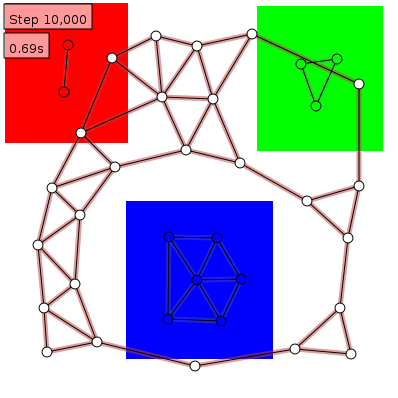
\includegraphics[width=0.5\textwidth]{rgb_static.png}
  \end{center}
  \caption{Computer-generated static image with red, green, and blue blocks on a white background. GNG quickly and correctly categorizes image.}
  \label{fig:rgbStatic}
\end{figure}

The pictures below (figure \ref{fig:1-4papers}) contain the GNG trying to categorize one, two, three, and four sheets of purple paper on a tan table background. As we see, with the GNG set on reasonable default settings ({\bf see Apendix \ref{appendix:staticImgParams}}), the first three images are categorized very accurately. Indeed, the GNG very quickly distinguishes between background and foreground images and correctly identifies distinct sheets of paper. 

\begin{figure}[h!]
  \centering

  \subfigure[Categorization on one sheet.]{
    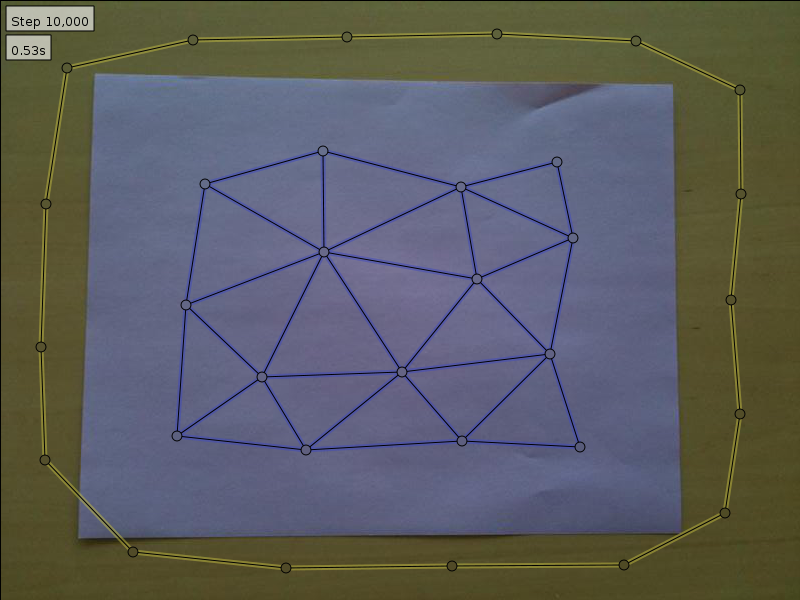
\includegraphics[width=0.45\textwidth]{paper1.png}
  }
  \subfigure[Categorization on two sheets.]{
    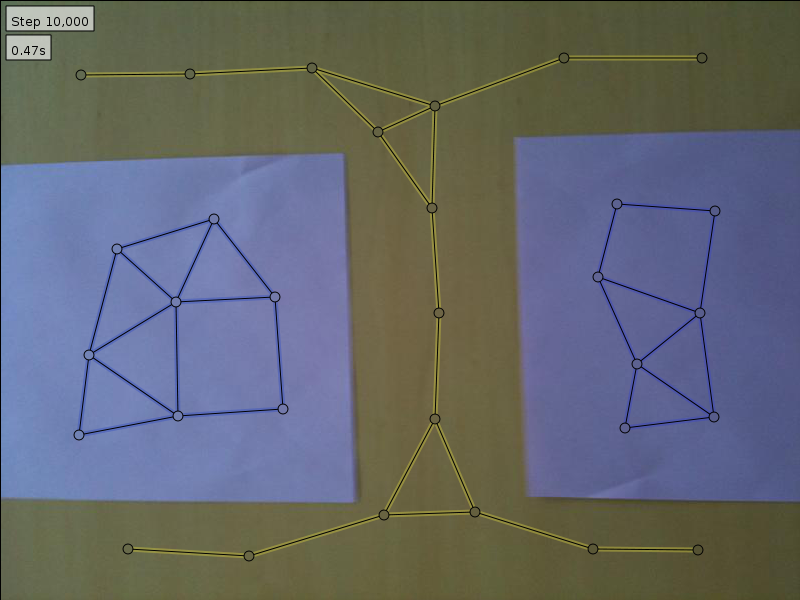
\includegraphics[width=0.45\textwidth]{paper2.png}
  }
  \subfigure[Categorization on three sheets.]{
    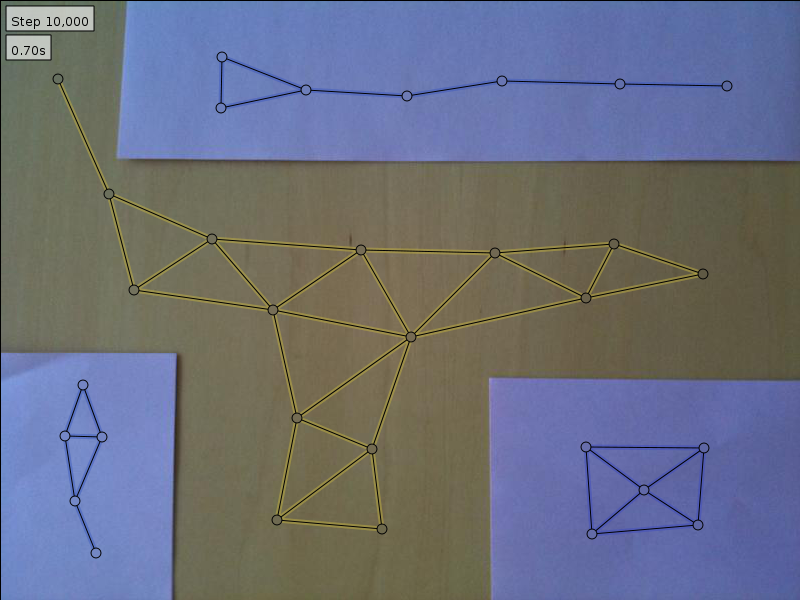
\includegraphics[width=0.45\textwidth]{paper3.png}
  }
  \subfigure[Categorization on four sheets.]{
    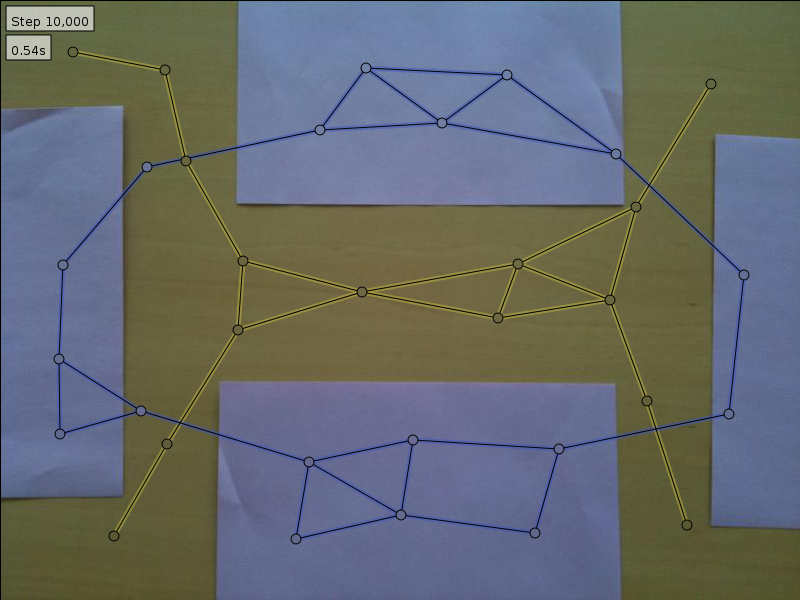
\includegraphics[width=0.45\textwidth]{paper4.png}
  }

  \caption{GNG categorizing sheets of purple paper on a table.}
  \label{fig:1-4papers}
\end{figure}

The final image with four sheets, however, is not correctly categorized. The GNG contains only two disjoint subgraphs instead of five. The table is correctly identified, but all four sheets of paper are part of the same subgraph. We show the result after 10,000 iterations, but given any number of iterations the graph's basic structure does not change. This is the result of the target error being too high so the GNG does not need add more nodes to better fit the object space. We expect that lowering the target error will cause the GNG to create more nodes and better categorize the space. In \ref{fig:paper4Lowerror} we lower the target error from 0.05~to~0.01 and we see a marked improvement. The image in figure \ref{fig:paper4_10,000} the represents the GNG after 10,000 iterations (the same number of iterations as before). We see the GNG is beginning to create disjoint subgraphs but has not yet accurately categorized the object space. After 20,000 iterations (figure \ref{fig:paper4_20,000}), however, the GNG has fully and correctly broken the image up into five distinct subgraphs that we can track. Thus, by lowering the target error we can more accurately describe a space, but it comes with a time cost. 

\begin{figure}[h!]
  \centering
  \subfigure[Categorization after 10,000 steps.]{
    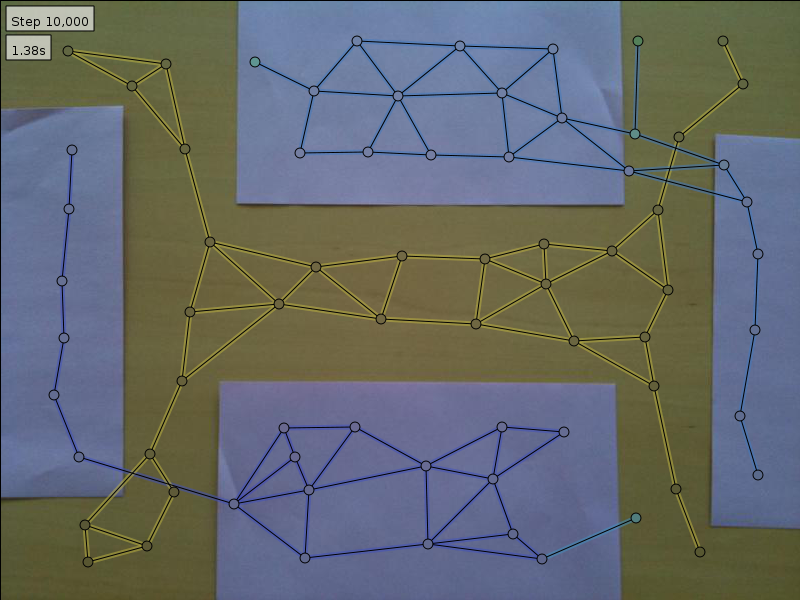
\includegraphics[width=0.45\textwidth]{paper4_lowerror10000steps.png}
    \label{fig:paper4_10,000}
  }
  \subfigure[Categorization after 20,0000 steps.]{
    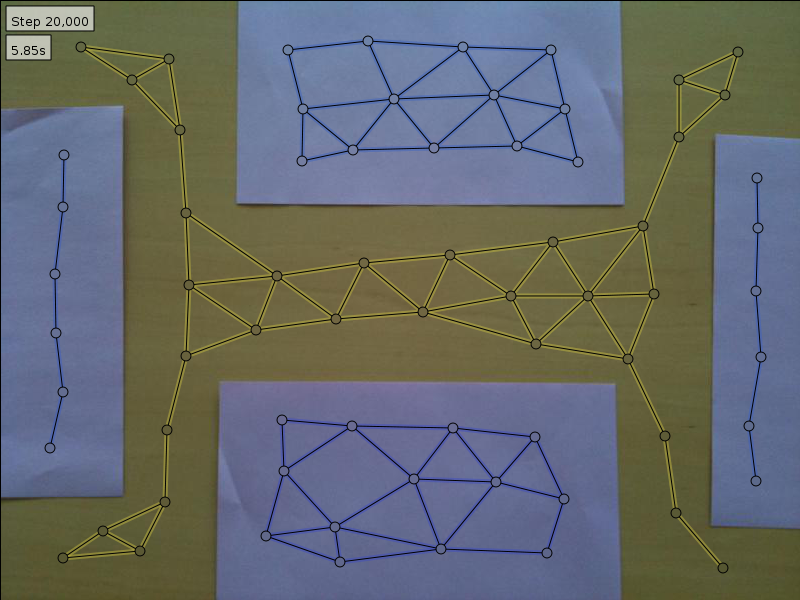
\includegraphics[width=0.45\textwidth]{paper4_lowerror20000steps.png}
    \label{fig:paper4_20,000}
  }

  \caption{GNG correctly categorizing four sheets of paper with adjusted error.}
  \label{fig:paper4Lowerror}
\end{figure}

\subsection{Moving Images}

%GNG is able to follow what's going on. Very cool!
We have also experimented with tracking objects in moving images. Here we again consider computer-generated sequences of images and real-life video, taken from a webcam. In figure \ref{fig:rgbMoving} we see the familiar image with red, green, and blue blocks on a white background. This time, however, the red block moves towards the center of the scene and then outward back to its original position. The GNG is able to quickly categorize the red block and then follow it as it travels around the scene. Note also that in addition to the green and blue blocks having stable categorizations throughout the experiment, the white background nodes moved out of the way as the red block moved. This is encouraging, showing that the GNG is able to adapt over time.

\begin{figure}[h!]
  \centering
  
  \subfigure[Red block in upper left corner.]{
    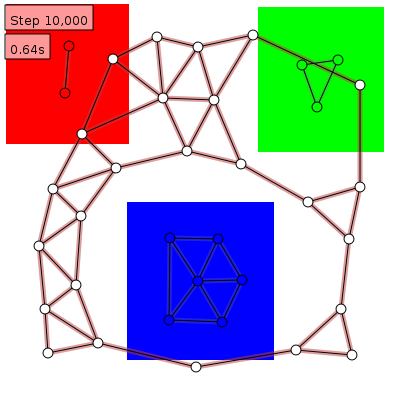
\includegraphics[width=0.45\textwidth]{rgb_motion1.png}
  }
  \subfigure[Red block moving towards center.]{
    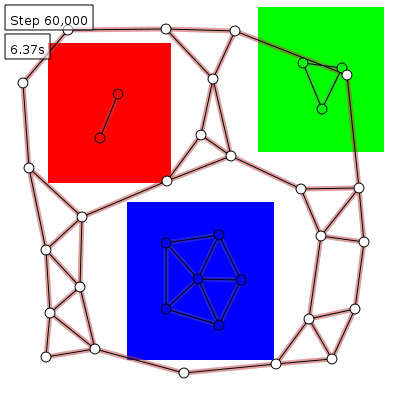
\includegraphics[width=0.45\textwidth]{rgb_motion2.png}
  }
  \subfigure[Red block at center of scene.]{
    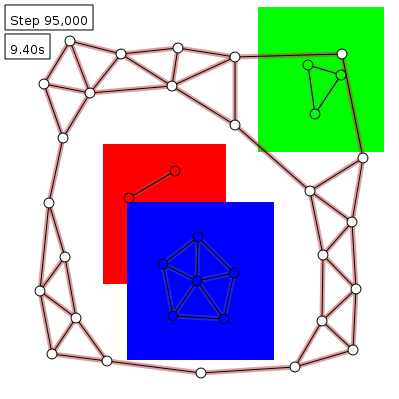
\includegraphics[width=0.45\textwidth]{rgb_motion3.png}
  }
  \subfigure[Red block returning to upper left corner.]{
    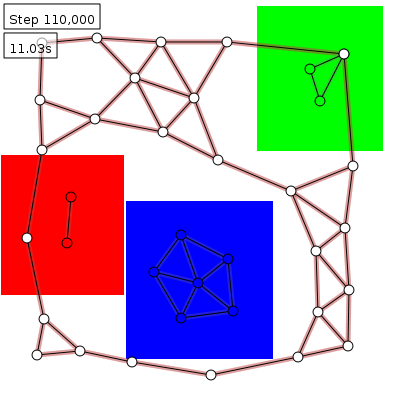
\includegraphics[width=0.45\textwidth]{rgb_motion4.png}
  }
  
  \caption{GNG categorizing a red block moving through a scene.}
  \label{fig:rgbMoving}
\end{figure}

A webcam was also used to see how the GNG dealt with real-time updates from noisy data. Results here were less successful that in past trials but still very encouraging. When presented with clear foreground objects and a distinct background, the GNG was able to correctly classify various foreground objects. On the other hand, complex scenes like faces or full room views were very difficult for the GNG to categorize. In figure \ref{fig:webcam} we placed an arm wrapped in a black cloth in front of a whiteboard with carefully controlled lightening. The GNG was able to quickly (within three seconds) identify the basic shape of the arm but it took a full ten seconds before clear and distinct subgraphs between background and foreground emerged. As with the colored blocks above, as the arm moves through the scene the background categorization moves out of the way to make space.

\begin{figure}[h!]
  \centering
  
  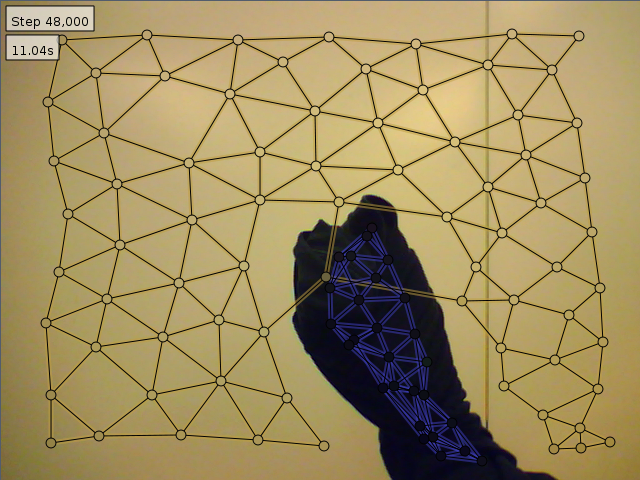
\includegraphics[width=0.45\textwidth]{webcam.png}
  
  \caption{GNG categorizing a webcam image.}
  \label{fig:webcam}
\end{figure}

\subsection{Real-Time Object Tracking with AIBO}

% Here's where the implicit memory really helps. As objects move and disappear, GNG is able to cull useless errors.
We were able to interface with the AIBO using libraries we created in C++ to make the robot turn its head appropriately as an image being tracked moves around the scene. Initially we tried using the ABIO's built-in camera but grabbing images over the wireless connection kept the semaphore locked for too long and thus caused the gngviewer to update slowly and irregularly. This made experimentation very difficult using only tools available to the AIBO. As a proof of concept, to show our GNG could correctly track objects, we instead used the webcam and pretended it was the AIBO's camera. That is, when an object moved to the left of the scene, we caused the AIBO to turn its head to the left. When an object moved back to the center, the AIBO returned its head to the forward position.

Our experiment consisted of a black wallet on a white background. The wallet would be selected as the object to follow by the following process. We specified that we wanted to follow {\em some} black object. Once the subgraphs had been generated, the subgraph with the average color closest to black was chosen as the object to follow. As the subgraphs change, the designated follow subgraph changes with it. At any time we can query the ``center'' of the subgraph, which calculates the average of all the $(x,y)$ points in the subgraph. We can use this average to figure out which of six quadrants the object is currently in. There are left, middle, and right sections and each of those can be broken into top and bottom sections. Provided the object was not moved too quickly, we were able to successfully ``track'' the object by making the AIBO's head turn appropriately. When the follow object moved too quickly, many nodes that used to be part of the object moved into the background and we switched to following the background, which isn't very useful. We discuss this in more depth in section \ref{sec:future}.

\subsection{Limitations}

No sense of edges or depth, so we perform poorly on complex, busy images. Example of busy image? Computer in Stromme's room?

\section{Future Work}
\label{sec:future}

\begin{itemize}
  \item Reduce resolution
  \item Black and white only
  \item make error more precise as time goes on if not enough subgraphs
  \item more robust AIBO object-following mechanisms
\end{itemize}

\appendix
\section{Default Parameters for Static Images}
\label{appendix:staticImgParams}

\end{document}
